\documentclass[10pt,twocolumn,letterpaper]{article}

\usepackage{cvpr}
\usepackage{times}
\usepackage{epsfig}
\usepackage{amsmath}
\usepackage{amssymb}
\usepackage{xcolor}
\usepackage{graphicx}
\usepackage{caption} 
\usepackage{subcaption}
\captionsetup[table]{skip=8pt}
\usepackage[normalem]{ulem}

% Include other packages here, before hyperref.

% If you comment hyperref and then uncomment it, you should delete
% egpaper.aux before re-running latex.  (Or just hit 'q' on the first latex
% run, let it finish, and you should be clear).
\usepackage[pagebackref=true,breaklinks=true,colorlinks,bookmarks=false]{hyperref}

\def\R{\mathbb{R}}
\newcommand{\red}[1]{\textcolor{red}{#1}}

\cvprfinalcopy % *** Uncomment this line for the final submission

\def\cvprPaperID{****} % *** Enter the CVPR Paper ID here
\def\httilde{\mbox{\tt\raisebox{-.5ex}{\symbol{126}}}}

% Pages are numbered in submission mode, and unnumbered in camera-ready
\ifcvprfinal\pagestyle{empty}\fi
\begin{document}

%%%%%%%%% TITLE
\title{%
  Visual Grounding of Phrases with Scene Graph Embeddings \\
  \large CPSC 532S, 2018W2, Project Report}

\author{Zicong (Alex) Fan\\
University of British Columbia\\
Computer Science\\
{\tt\small fan@cs.ubc.ca}
% For a paper whose authors are all at the same institution,
% omit the following lines up until the closing ``}''.
% Additional authors and addresses can be added with ``\and'',
% just like the second author.
% To save space, use either the email address or home page, not both
\and
Si Yi (Cathy) Meng\\
University of British Columbia\\
Computer Science\\
{\tt\small mengxixi@cs.ubc.ca}
}

\maketitle
%\thispagestyle{empty}

\section{Introduction}
Visual grounding is the task of associating textual input with the corresponding regions in a given image. The problem has attracted much attention in recent years as it plays an important role in applications such as image retrieval and intelligent dialogue systems. Many of the recent works such as \cite{rohrbach2016grounding, deng2018visual} perform visual grounding by utilizing unstructured visual features from pretrained object classification networks such as VGG16 \cite{simonyan2014very}. However, in reality, the representation of an object in a scene should be structurally constrained by its surroundings. As an example, the feature representation of ``a man sitting alone in a bus" should be inherently distinct from the same man ``sitting on the beach with his family". 

This observation motivates our work on augmenting visual grounding systems with scene graph embeddings. Unfortunately, most datasets in the computer vision community do not come with scene graphs that annotate relationships between objects in an image. Some prior works such as \cite{teney2017graph} in visual question answering attempted to encode relationship between objects by relying solely on spatial relationships (such as relative positions of bounding boxes). However, spatial information might not be sufficiently rich in expressing contextual pairwise relationships between objects. On the other hand, there have been on-going research in scene graph generation which attempt to assign more meaningful predicate relationships between objects in an image \cite{xu2017scene, zhang2017relationship, yang2018graph, NIPS2018_7951, gu2019scene} . Therefore, in this work, we propose a method that enhance visual grounding by incorporating scene object embeddings through an auxiliary scene graph generation task. 

Our contributions are summarized as follows. First, we show that the use of scene graph embedding can significantly improve the performance of a simple visual grounding system, and our proposed model achieves an accuracy close to that of the state-of-the-art. We perform ablation studies to demonstrate the impact of adopting our framework, and finally we explore the possibility of augmentation with sentence graphs as well as multi-instance grounding.
%------------------------------------------------------------------------
\section{Related Work}
\subsection{Visual Grounding}
\label{sec: vg_attention}

Many approaches have explored using attention with different levels of granularity in the visual grounding task. In particular, \cite{rohrbach2016grounding} applies attention weights on the aggregated features of proposal bounding boxes and input phrases, and attempts to reconstruct the phrase using these attention weights. The loss is applied on the reconstructed phrase, and hence the attention weights will be maximized for the correct box. \cite{xiao2017weakly} instead performs grounding at the pixel level with spatial attention masks without any explicit bounding box annotations. The spatial attention masks are generated by exploiting the hierarchical structure of the parse tree from an image caption. In order to enforce joint learning on the multimodal input source, \cite{deng2018visual} applies attention on the query, image and object regions simultaneously to obtain a more compact correspondence between the correct pairs. In a recent work, \cite{dogan2019neural} formulates grounding of phrases in a sequential and contextual manner, leveraging comprehensive global information, and enabling well performing multi-instance grounding.

\subsection{Multimodal Learning with Graph Embeddings}
The omnipresence of graph structured data has promoted considerable research effort devoted to representation learning of the graph nodes. The goal is to project node features onto a latent space while preserving the pairwise relationship encoded in the underlying graph. These embeddings can then be used in various downstream machine learning tasks such as node classification, link prediction and neighborhood identification \cite{hamilton2017representation}. Recent works often use a deep neural network architecture which allows node features to be incorporated into the embeddings. One of the most popular approaches is to use a neighborhood aggregation function (similar to message-passing) to learn a local representation, possibly inspired by convolutional filters in computer vision. In particular, the graph convolutional network (GCN) was introduced to perform transductive learning with node features and the graph's adjacency matrix \cite{kipf2016semi}.


Several works have taken advantage of an underlying graph structure of a problem in a multimodal learning setting. In the task of visual question answering, \cite{teney2017graph} encodes both the question and the input scene image as separate graphs that capture the spatial arrangement and contextual information to enhance their prediction over the output vocabulary. However, this method requires knowing the image regions of interest and their pairwise relationships beforehand, which are often unavailable in a real-world setting. To overcome this problem, scene graph generation networks such as \cite{yang2018graph} has been proposed, which motivates our work to improve visual grounding systems using scene graph embeddings. 

\subsection{Scene Graph Generation}

Visual scene graph generation is a task that requires not only accurately detecting objects in an image, but also correctly predicting the subtle interactions between them. The vertices in a scene graph are the individual scene object bounding boxes, while the edges represent their relationships as predicates. For instance, in an image depicting ``a man wearing a shirt sitting on a bench", the corresponding scene graph should have vertices \texttt{\{Man, Shirt, Bench\}} and edges \texttt{\{(Man, Wearing, Shirt), (Man, Sitting, Bench)\}}. Recently, \cite{xu2017scene} proposed a message passing architecture utilizing messages with contextual information between a pair of bipartite graphs, of which the set of edges are refined iteratively. \cite{zhang2017relationship} developed a Relationship Proposal Network (Rel-PN) that directly predicts relationships by scoring the likelihood of the triplet \texttt{(subject, object, and relation)}. \cite{yang2018graph} designed a Relation Proposal Network (RePN) that proposes potential edges among object bounding boxes and uses an attentional GCN (aGCN) model to aggregate node and edge features to generate scene graph.  \cite{gu2019scene} tried to tackle issues from noisy and biased annotations in the Visual Genome dataset \cite{krishna2017visual} by regularizing the model via reconstructing the original image from scene graph predictions. \cite{NIPS2018_7951} formulated the scene graph generation task as a score-based structure prediction problem and designed a network so that it is invariant to permutation in the input structure. 


%------------------------------------------------------------------------
\section{Our Approach: GraphGround}
\begin{figure}
    \centering
    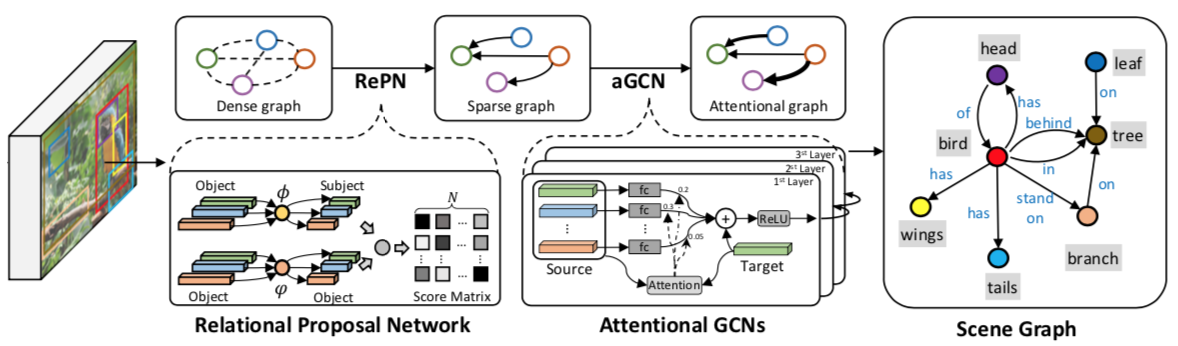
\includegraphics[width=0.5\textwidth]{latex/figures/graphrcnn_framework.png}
    \caption{Graph R-CNN Pipeline, illustration from \cite{yang2018graph}.}
    \label{fig:graphrcnn_framework}
\end{figure}

% Figure \ref{fig:graphrcnn_framework} shows the Graph R-CNN architecture.
We leverage the Graph R-CNN architecture for scene graph generation to learn a graph representation over the proposed regions. Our re-implementation follows the original work of \cite{yang2018graph} (see Fig. \ref{fig:graphrcnn_framework}) with minor modifications. Given an image $I$, we use Faster R-CNN \cite{ren2015faster} to generate bounding boxes $r_i = [x_i, y_i, w_i, h_i]$  around potential objects, along with their associated visual features $X_i \in \R^d$ and the distribution over label classes $P_i \in \R^c$. Here $i$ denotes the index of an arbitrary bounding box, $d$ is the visual feature dimension and $c$ is the number of object label classes. Then the RePN uses a learned asymmetric kernel function $\phi(P_i, P_j)$ to predict whether there should be a directed edge from $r_i$ to $r_j$, and incorrect edge assignments are penalized using a binary classification loss function. This gives us a graph with $n$ vertices (proposed bounding boxes) and $m$ edges (proposed relationships). The visual features $X_{ij}$ associated with the union of $r_i$ and $r_j$ are extracted as the initial edge features. Given the graph with its initial features $X_i$ and $X_{ij}$, an attentional GCN (aGCN) performs graph convolutions on the proposed graph to aggregate both node features and edge features.  The aGCN is a variant of GCN \cite{kipf2016semi} with the additional use of a weighted average during neighborhood aggregation based on attention scores. Finally, the node and the edge features are mapped to the node and edge label space respectively, where incorrect classifications are penalized via another loss function. 

For the downstream visual grounding task, our model is inspired by the supervised version of GroundeR \cite{rohrbach2016grounding}, where each query consists of a scene image and a phrase to be grounded, as well as the the groundtruth bounding box. We first extract the visual features of 100 proposed bounding boxes of the image and project them to a lower dimension $d$. The query phrase is encoded using a language model then fed into a LSTM, of which the hidden states are also projected to a $d$-dimensional latent space. After batch normalization, we sum the visual features with the hidden state of the LSTM, which then goes through an activation and finally projected onto the output label space, which consists of our bounding box proposals. This last layer is referred to as the ``attention"  \cite{rohrbach2016grounding} , which we can normalize using softmax and choose the index that gives rise to the highest probability as the predicted proposal index. The target proposal index corresponds to the proposal bounding box with the highest IoU (intersection over union) with the groundtruth bounding box (out of all proposed bounding boxes that has a $>$ 0.5 IoU with the groundtruth). This way, the grounding task simply boils down to an ordinary multi-class classification problem.

Instead of using visual features extracted from a pre-trained image classification network that neglects pairwise scene object interactions, we use the logits at the end of the aGCN of our Graph R-CNN model as the visual features. This way, the features have been optimized to preserve the pairwise relationship between scene objects, and thus provide a more comprehensive representation of the proposals to be grounded. Intuitively, suppose that there are two proposal bounding boxes that both capture ``hands" in a similar posture, but are from two different people. In this case, visual features from a generic image classification network would treat the two proposals independently, hence giving similar visual features due to their pixel-level similarity. However, visual features from the scene graph embeddings should ideally be much more different, as the relationship between scene objects are constraining the objects to be more distinguishable. Since the grounding benchmark dataset Flickr30k Entities \cite{plummer2015flickr30k} does not provide scene graph annotations, we use the Visual Genome dataset \cite{krishna2017visual} to pre-train our Graph R-CNN model, and then generate scene graphs on the Flickr30k Entities images to provide bounding box proposals as well as enhanced visual features. 

\section{Experiments and Results}
\subsection{Graph R-CNN}
\subsubsection{Dataset}
We use the Visual Genome dataset \cite{krishna2017visual} to train and benchmark our Graph R-CNN model. Since training a Faster R-CNN from scratch takes several days and our pretrained backbone uses a data split that is different from that of the original Graph R-CNN paper \cite{yang2018graph}, we decided against re-training on the exact same split solely for benchmarking purposes. Our goal is to use the learned scene graph embeddings for the downstream grounding task, hence a satisfactory performance on an arbitrary data split should justify its use in the downstream task. The data split we used consists of $98,077$ training images, $5,000$ validation images and $5,000$ test images. Following the same scene graph preprocessing procedure as \cite{yang2018graph}, the top-frequent 150 object labels and 50 relationship predicate labels are chosen. Bounding boxes and predicates that are out-of-vocabulary are removed. Additionally, a relationship predicate is removed if either of its connecting bounding box is removed. 

\subsubsection{Implementation} 
Since we do not have access to a working open source implementation of Graph R-CNN nor a pretrained model, we need to provide our own implementation. Based on the Faster R-CNN implementation in \cite{jjfaster2rcnn}, using a pretrained VGG16\cite{simonyan2014very} backbone, we train the rest of the network while freezing the backbone and finetuning the object detector for 47 epochs until convergence. We use the SGD \cite{robbins1951stochastic} optimizer with a learning rate of 0.0001 and a batch size of 2 (small batch size due to hardware constraints). We randomly flip training images horizontally for data augmentation and variability. We use a threshold of 0.6 for  the non-maximal suppression (NMS) of the bounding boxes, and 100 region proposals are returned per image. All hyper-parameters are chosen based on the validation set. Finally, with our trained Faster R-CNN network, we are able to obtain an mAP score of 0.125 using an IoU 0.5 threshold for box alignment. The bounding boxes $r_i$, the probability distribution $P_i$, and the box feature $X_i$ are extracted as input to rest of the Graph R-CNN modules. 

Since every image may have a different number of groundtruth bounding boxes (thus a different number of possible edges), we pick the top $k\%$ (ranked by their predicted scores) of the $n^2$ edges rather than an exact number $k$. Based on our validation set edge recall, we choose $k$ to be $3\%$. We also set the scores of edges representing self-loops to zero as they are of little interest in this task. Additionally, since most adjacency matrices of scene graphs are relatively sparse, there is heavy class imbalance in the binary classification of edge proposal. To alleviate this problem, when computing the loss during training, we compute the fraction $p$ of positive class in the adjacency matrix and assign a weight of $1/p$ to the positive examples and  $1/(1-p)$ to the negative examples. For the aGCN implementation, the original paper recommends adding ``skip connections" between all bounding boxes, resulting in a fully connected graph for better information flow \cite{yang2018graph}. However, we do not include these as empirically they provide little improvement to the bounding box and predicate classification accuracy. Finally, we train the aGCN using groundtruth scene graph from Visual Genome. Our first attempt was to train the RePN and aGCN jointly with only one loss function at the end, but we settled on training the two modules each with their own supervision mainly due to an empirical degradation in the evaluation metric SGGen and SGGen+. Another reason is the fact that the Graph R-CNN architecture is not fully differentiable, due to the top $k\%$ edge selection at the end of RePN. Also, when RePN predicts an edge that does not belong to the groundtruth edge set, the groundtruth predicate labeling for that edge would not be well-defined. Thus, only the predicted edges that align with the groundtruth can be propagated. We tried to allow the joint training of RePN and aGCN by assigning the label \texttt{no\_relation} to the edges that do not align with a groundtruth, but we find that this deteriorates the performance. Lastly, NMS is a slow operation, training the modules with separate supervision allows us to persist the results from RePN, thus avoiding running NMS at every aGCN training iteration.

In detail, RePN's two branches of the asymmetric kernel function $\phi(P_i, P_j)$ have the same structure with input dimension 155, hidden layer dimension 256 and output dimension 64. We use $\tanh(\cdot)$ as the  activation function. The input features contains the probability in the 151 label categories (including a \texttt{background} label) and the spatial information $(x, y, w, h)$ of bounding boxes. Specifically, the $x, y$ values are normalized to be between 0 and 1. Each of edge and node convolution of aGCN contains 2 aGCN layers with the input size 256, hidden size 512 and output size equal to the number of categories in each label space. Each linear layer are separated using $tanh(\cdot)$. Both models are trained with the Adam optimizer \cite{kingma2014adam} with a learning rate of 0.0001 and no batching for simplicity. The RePN is trained for 15 epochs while the aGCN is trained for 5 epochs. 

\subsubsection{Discussion}
Table \ref{tab: sggen} shows the results of our model on Visual Genome. We follow the same convention in the literature by computing the ``recall at 50" (abbreviated as R@50) and ``recall at 100" metric score. For example, ``R@50" means that we sort all triplet predictions by the product of three classification confidence scores (two boxes and one predicate) in descending order and evaluate the score of the top-50 predictions. From Table \ref{tab: sggen}, we can see that our model works well in object recall, which results in a higher SGGen+ score while the low SGGen score is due to a lower recall in the predicates. It makes sense since relationship proposal is a less well-defined problem. 

\begin{table}[]
\begin{tabular}{|l|c|c|c|c|}
\hline
\multicolumn{1}{|c|}{Models/Metric} & SGGen+        & SGGen & PredR & ObjR \\ \hline
Original (R@50)                     & 28.5          & 11.4  & -     & -    \\ \hline
Original (R@100)                    & 35.9          & 13.7  & -     & -    \\ \hline
Ours (R@50)                         & \textbf{32.5} & 4.6   & 10.9  & 45.1 \\ \hline
Ours (R@100)                        & 33.1          & 5.9   & 13.1  & 45.1 \\ \hline
\end{tabular}
\caption{Graph R-CNN performance on Visual Genome dataset. Let $C(\cdot)$ denote a count operation, $O, P, T$ denote correct object, predicate (two boxes correctly localized), and triplet (two boxes correctly localized and labeled) predictions. SGGen+ is computed as $(C(O)+ C(P)+C(T))/N$ where $N$ is a normalizing constant; SGGen is computed by $C(T)/N'$ where $N'$ is number of groundtruth predicates; the other two metrics are predicate and object recall rates. Groundtruth and predicted boxes are aligned if they have $>0.5$ IoU.}
\label{tab: sggen}
\end{table}

\subsection{Grounding}
\subsubsection{Dataset}
The Flickr30k Entities dataset \cite{plummer2015flickr30k} contains 31,783 images in total. Each image has 5 sentences that contain phrases describing entities in the image that can be grounded. Each phrase is also annotated with the groundtruth bounding boxes within the image. To be consistent with previous work, we use the same data split provided, which consists of 1000 images for validation, 1000 images for testing, and the rest for training. At evaluation time, a predicted bounding box that has a $>$ 0.5 IoU with the groundtruth bounding box is considered correctly grounded, and we report the accuracy on the test set, which is the percentage of the test set phrases that are correctly grounded. 

\subsubsection{Implementation and Results}


To encode the query phrase, we use 200-dimensional GloVe \cite{pennington2014glove} embeddings pretrained on the Twitter corpus. A dropout with probability 0.5 is applied to the word embeddings before being fed into a 1-layer, uni-directional LSTM with hidden size 200. The hidden states are then batch-normalized and projected to 128 dimension. As a baseline, we first use the 4096-dimensional features extracted from the fully connected fc7 layer of a VGG16 network\cite{simonyan2014very} trained on ImageNet \cite{krizhevsky2012imagenet}. This also serves as the basis of an ablation where we compare our results when scene graph features are included. We have also experimented using only the 512-dimensional scene graph features extracted from Graph R-CNN, as well as concatenating scene graph features with the VGG features as augmented visual features. The visual features also have a 0.5 dropout applied, batch normalized and projected to 128 dimension, which are then summed with the projected hidden states from the phrase. The aggregated features then go through a ReLU activation followed by a fully connected layer that forms the attention over the proposed bounding boxes. We train our grounding model for 40 epochs with batch size 64. We use the Adam optimizer \cite{kingma2014adam} with a learning rate of 0.001 that decays by 0.1 at epoch 15 and 25. In addition to the dropout layers, we apply a weight decay of 0.0005 to further prevent overfitting.

\begin{table*}[t]
\centering
\begin{tabular}{lll} 
\hline
\textbf{Approach}                             & \textbf{Accuracy}  & \textbf{Proposal upper bound}   \\ 
\hline
\textbf{Other work}                           &                    &                                 \\
GroundeR \cite{rohrbach2016grounding}                                      & 47.8               & 77.90                           \\
SeqGround \cite{dogan2019neural}                                    & \textbf{61.6 }     & -                             \\
\hline
\textbf{Ours}                                 &                    &                                 \\
Baseline (VGG features only)                  & 31.1               & 86.0                            \\
VGG+Scene graph features                      & \textbf{58.4 }     & 86.0                            \\
Scene graph features only                     & 56.9               & 86.0                            \\
Scene graph + Sentence graph (simple average) & 55.8               & 86.0                            \\
Scene graph + Sentence graph (sentence GCN)   &51.0                    & 86.0                            \\
\hline
\end{tabular}
\caption{Phrase grounding accuracy (in \%) on Flickr30k Entities test set with comparison to state-of-the-art results. The proposal upper bound is the proportion of correct bounding boxes (overlaps with groundtruth with IoU $>$ 0.5) among the proposals.}
\label{tab: grounding}
\end{table*}

The results are shown in Table \ref{tab: grounding}. As we can see, with the addition of scene graph embeddings, our accuracy has significantly improved over our baseline, and our results are fairly close to the accuracy in \cite{dogan2019neural}, the state-of-the-art work in visual grounding. In addition, the scene graph features alone can already provide us with significantly better visual representation of the proposals, as seen from the results. We also present some qualitative results in Figure \ref{fig: qualitative}. 

\begin{figure*}[t]
  \begin{subfigure}[t]{.32\linewidth}
    \centering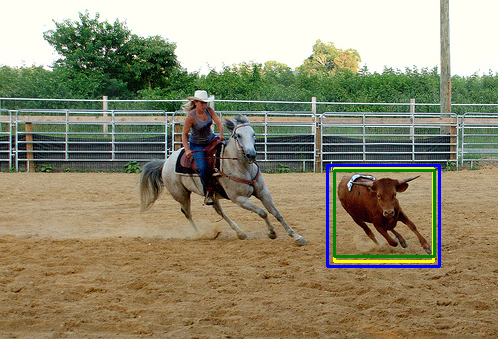
\includegraphics[width=1\linewidth]{latex/figures/g5.png}
    \caption{a calf}
  \end{subfigure}\hfill
    \begin{subfigure}[t]{.32\linewidth}
    \centering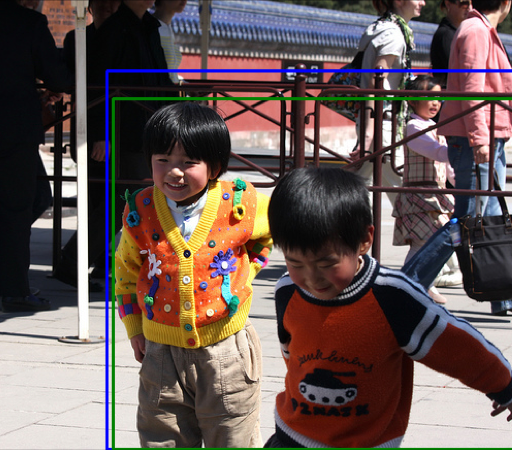
\includegraphics[width=1\linewidth]{latex/figures/g2.png}
    \caption{Two children}
  \end{subfigure}\hfill
    \begin{subfigure}[t]{.32\linewidth}
    \centering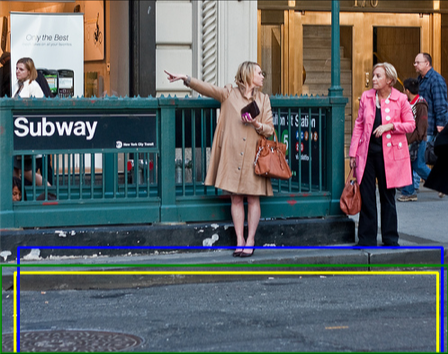
\includegraphics[width=1\linewidth]{latex/figures/g3.png}
    \caption{the street}
  \end{subfigure}
  \par\medskip
  
  \begin{subfigure}[t]{.32\linewidth}
    \centering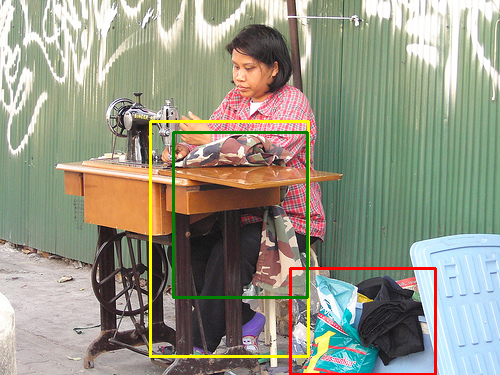
\includegraphics[width=1\linewidth]{latex/figures/b4.png}
    \caption{a camouflage colored garment}
  \end{subfigure}\hfill
    \begin{subfigure}[t]{.32\linewidth}
    \centering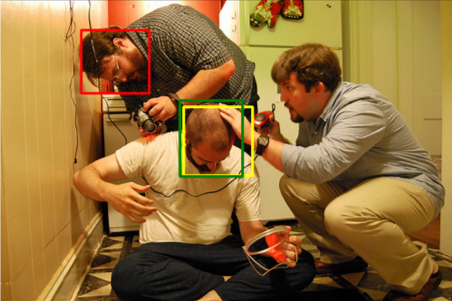
\includegraphics[width=1\linewidth]{latex/figures/b2.png}
    \caption{a haircut}
  \end{subfigure}\hfill
    \begin{subfigure}[t]{.32\linewidth}
    \centering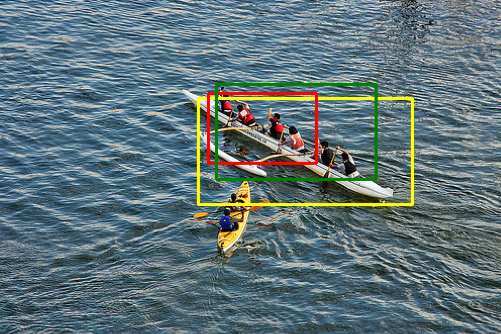
\includegraphics[width=1\linewidth]{latex/figures/b3.png}
    \caption{six rowers}
  \end{subfigure}

  \caption{Sample results obtained with our model using VGG+Scene graph features. The green boxes are the groundtruth boxes. Yellow boxes represent the target proposal that overlaps the most with the groundtruth. Blue boxes are correctly grounded proposal bounding boxes, while red boxes are incorrectly grounded (has an IoU $\leq$ 0.5 with the groundtruth (best viewed in color).}
  \label{fig: qualitative}
\end{figure*}

\subsubsection{Negative Results and Discussion}
\textbf{Sentence Graph: }
So far, we have been treating query phrases as independent entities regardless of its residing sentence, neglecting information in the overall semantic structure. In attempt to further enhance our grounding results, we construct a dependency graph over each sentence using the Stanford dependency parser \cite{de2008stanford}. The dependency graph is represented using an undirected, unweighted adjacency matrix, where an edge represents the existence of a semantic dependency between the two tokens. 

Our first experiment in this direction involves averaging a word's embedding with its neighbours based on the sentence graph to incorporate dependent words' information into the phrase. This approach should provide an advantage at inference time where the query phrase contains out-of-vocabulary words when the language model has a fixed-size vocabulary determined at training time. In this situation taking the neighbours into account should provide some information about the phrase being grounded rather than having no available information at all. 

Our second approach to incorporating sentence structure into grounding is to pre-train a sentence reconstruction model using the scene image features as well as the sentence dependency graph. The reconstruction model has a 2 layer GCN that operates over the sentence dependency graph with GloVe\cite{pennington2014glove} embeddings as initial node features. The convolved embeddings are then passed into an LSTM encoder. We also extract visual features for the entire scene using the same VGG16\cite{simonyan2014very} network, and concatenate that with the encoder LSTM's hidden states, and use the concatenated features as the initial hidden states of a LSTM decoder. The decoder's goal is to use the encoded features from the sentence graph as well as the scene image to reconstruct the sentence back.

The results are shown in the last two lines of Table \ref{tab: grounding}. As we can see, the inclusion of sentence graph has worsened our accuracy, however, this is unsurprising to some extent. Recall that there are 5 annotated sentences corresponding to each image, which means that there could be potentially multiple identical query phrases with the same groundtruth bounding boxes (see Fig \ref{fig: sentence}). This particular structure of the dataset introduces a large number of ``duplicate" data pairs when each phrase is encoded using a language model independent of the sentence it belongs to. These duplicate pairs are easier to ground as the training data also contain duplicate pairs of a similar type (e.g. subjects of a sentence), and it also means that once we can correctly ground one of these duplicate phrases for a test image, we automatically ground correctly for the rest of them. Although incorporating sentence-level structure should intuitively improve grounding accuracy by using a more sophisticated, context-dependent phrase representation, this approach is in fact perturbing the dataset that was not independently and identically distributed in the first place. However, we believe with more tuning, we should still be able to achieve better results with the use of sentence graphs, but in the interest of time we performed minimal tuning in this direction. 

\begin{figure}[t]
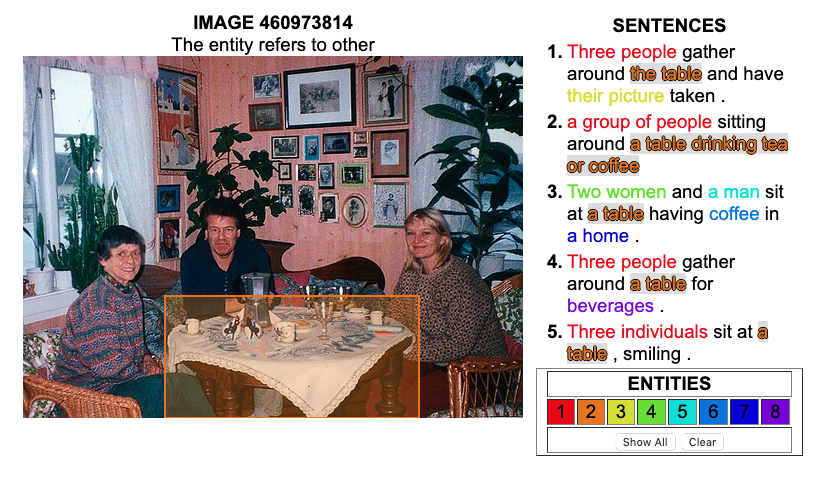
\includegraphics[width=8cm]{latex/figures/sentence.png}
\caption{Without sentence-level context, we will have 3 identical data pairs with query phrase ``a table" corresponding to the same groundtruth bounding boxes. Image taken from \cite{plummer2015flickr30k}  (best viewed in color).}
\label{fig: sentence}
\centering
\end{figure}

\textbf{Multi-instance Grounding: }
Following prior work, when there are multiple groundtruth boxes for a query phrase, we take the union by merging all into one big box (by taking the minimum upper left coordinate and the maximum bottom right coordinate) and take that as the groundtruth target. We refer to this as the \textit{axis-aligned convex hull union}. But this approach can misrepresent the actual groundtruth in many cases (see Fig \ref{fig: multiinstance}). In addition, by taking the union this way, most existing work predicts only one bounding box per query phrase, which is a very crude approach. It is worth noting that in \cite{dogan2019neural}, the authors are in fact performing multi-instance grounding, however, the axis-aligned convex hull union is still being used. We propose to take a more fine-grained union approach by treating the boxes as a grouped polygon, and the area where no boxes overlap is not counted towards the area. After we take the union of the groundtruth boxes, we also take the union of our predicted bounding boxes (in the multi-instance grounding experiment) and proceed with computing the IoU as a measure of performance. The IoU in this case would be a more representative and precise metric of how well the grounding model in fact performed. 

For multi-instance grounding, our naive approach is to cast the problem into a multi-label classification problem, where the predicted probability for each proposed bounding box is between 0 and 1, and we take all proposals with a probabiliy $>$ 0.5 to be the predicted boxes. However, our results are unsatifactory, possibly due to the limitations of the model. Nonetheless, we believe it is necessary for the community to adopt a more fine-grained approach to taking the union and perform multi-instance grounding for a better understanding of the task. 


\begin{figure}[t]
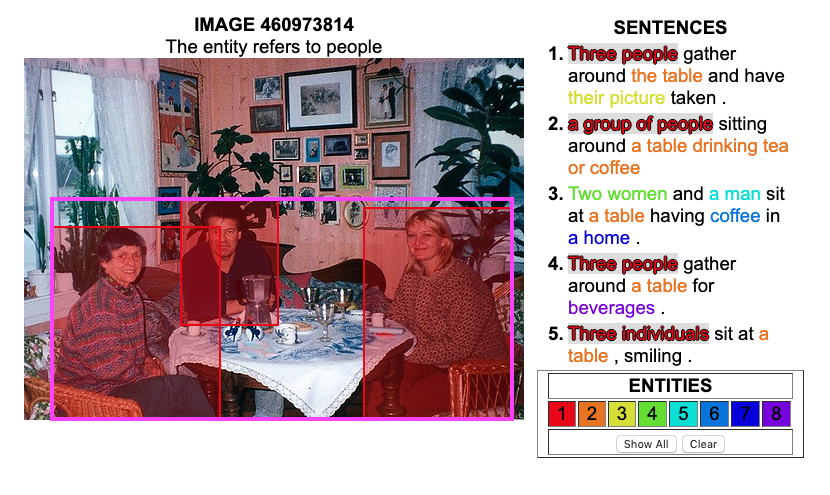
\includegraphics[width=8cm]{latex/figures/multiinstance.png}
\caption{When we try to ground ``Three people" in this image, our target proposal is the pink box using the union approach most widely adopted. However, this bounding box also captures the dining table, and thus is not an accurate reflection of the groundtruth. Image taken from \cite{plummer2015flickr30k}  (best viewed in color).}
\label{fig: multiinstance}
\centering
\end{figure}

\section{Conclusion}
To summarize our contributions, in this work, we demonstrate that the incorporation of scene graph embeddings can provide significant improvement to a simple grounding network. With our approach, we are able to achieve an accuracy that is very close to the state-of-the-art. We also point out an imperfection in the current way of treating multiple groundtruth adopted by the community, and propose to use a more fine-grained way of computing the evaluation metric. For the learning experience, this project has allowed us to gain more insight into machine learning with different modalities and expanded our knowledge in the area of representation learning on graphs. We also recognize the importance of code release with publication and its profound influence in the reproducibility of published results. In terms of work split, Alex focused on the implementation of Graph R-CNN, training and tuning on Visual Genome, and generating scene graph embeddings for the Flickr30k Entities dataset, while Cathy implemented the grounding framework and conducted various experiments with scene graph embeddings, sentence graphs and multi-instance grounding. Although our work seem to be on separate paths, we had many meaningful discussions when it came to bottlenecks for our own parts that were indispensable to this project.
{\small
\bibliographystyle{ieee}
\bibliography{egbib}
}

\end{document}
